\chapter{विक्षोभ सिद्धांत}\label{ch:b3:perturbation-theory}

मुट्ठी भर क्वांटम समस्याएँ ही ठीक-ठीक घुलती हैं: संदूक,
दोलक, हाइड्रोजन, द्वि-स्तरीय तंत्र। बाकी सब --- किसी क्षेत्र में कोई
परमाणु, किसी अणु का कड़ा पड़ता बंध, किसी पड़ोसी से ज़रा हटाया गया कोई
स्तर --- उन्हीं हल हो सकने वाले ढाँचों में से कोई है, जो एक छोटा
अतिरिक्त पद पहने हुए है। \omterm{thm:b3:perturbation-theory:corrections}{विक्षोभ सिद्धांत} उस अतिरिक्त पद को वही मानने
की कला है जो वह है: एक संशोधन, जिसे उसकी अपनी लघुता में
कोटि-दर-कोटि निकाला जाता है। उसका प्रथम-कोटि नियम एक पंक्ति का औसत है;
उसका द्वितीय-कोटि नियम समझाता है कि स्तर एक-दूसरे को \emph{ठेलते} क्यों
हैं, हर परमाणु ध्रुवणशील क्यों है, और वान डर वाल्स आकर्षण सार्वत्रिक
क्यों है; उसका अपह्रासी रूप उन नाज़ुक स्थितियों को सँभालता है जहाँ लगभग
बराबर स्तर पूरी तरह फिर से गढ़े जाते हैं; और उसका काल-निर्भर रूप ---
\omterm{thm:b3:perturbation-theory:golden}{फ़र्मी का स्वर्ण नियम} --- वही समीकरण है जो किसी भी प्रयोगशाला में नापी
गई हर अवशोषण-रेखा, क्षय-दर और प्रकीर्णन अनुप्रस्थ काट के पीछे है।
चलते-चलते के पुरस्कार के रूप में यह अध्याय आकाश का रंग निकालकर समाप्त होता है।

\section{छोटे खिसकाव: अ-अपह्रासी सिद्धांत}

\begin{theorem}[विक्षोभी संशोधन]\label{thm:b3:perturbation-theory:corrections}
\index{विक्षोभ सिद्धांत}
मान लीजिए $\hat H = \hat H_0 + \hat V$, जहाँ $\hat H_0$ हल हो चुका है
($\hat H_0\ket n = E_n\ket n$, वर्णक्रम अ-अपह्रासी) और $\hat V$
छोटा है। तब, $\hat V$ में कोटि-दर-कोटि,
\[
E_n' = E_n + \bra n\hat V\ket n
 + \sum_{m \neq n}\frac{|\bra m\hat V\ket n|^2}{E_n - E_m}
 + \cdots
\]
और अवस्था में मिश्रण आ जाते हैं: $\ket{n'} = \ket n + \sum_{m\neq
n}\dfrac{\bra m\hat V\ket n}{E_n - E_m}\,\ket m + \cdots$
\emph{प्रथम कोटि}: खिसकाव अविक्षुब्ध अवस्था में विक्षोभ का
औसत भर है। \emph{द्वितीय कोटि}:
दूसरे स्तरों से युग्मन $E_n$ को उनसे \emph{दूर} ठेलते हैं ---
ऊपर का हर $m$ नीचे ठेलता है, नीचे वाला ऊपर --- अतः मूल
अवस्था का द्वितीय-कोटि खिसकाव सदा ऋणात्मक होता है। वैधता: मिश्रण के
अंश $|\bra m\hat V\ket n/(E_n - E_m)|$ छोटे होने ही चाहिए।
\end{theorem}

\begin{proof}[आंशिक उपपत्ति]
$E' = E + \epsilon_1 + \epsilon_2 + \cdots$ और $\ket{\psi} =
\ket n + \ket{\psi_1} + \cdots$ का $\hat V$ की घातों में प्रसार कीजिए,
उन्हें $(\hat H_0 + \hat V)\ket\psi = E'\ket\psi$ में रखिए, और कोटियाँ
मिलाइए। प्रथम-कोटि समीकरण का $\bra n$ पर प्रक्षेप $\epsilon_1 =
\bra n\hat V\ket n$ देता है; $\bra m$ ($m \neq n$) पर प्रक्षेप
मिश्रण-गुणांक; और उन्हें द्वितीय-कोटि
समीकरण में ले जाकर फिर $\bra n$ पर प्रक्षेप करने से $\epsilon_2$ मिलता
है। मूल अवस्था के लिए चिह्न वाला कथन: हर हर $E_0 - E_m$
ऋणात्मक है, जबकि अंश वर्ग हैं।
\end{proof}

\begin{proposition}[एक ऐसा विक्षोभ जिसका यथार्थ उत्तर है]\label{prop:b3:perturbation-theory:oscillator-field}
आवेश $q$ के किसी दोलक का, किसी एकसमान क्षेत्र $\mathcal E$ में,
$\hat V = -q\mathcal E\hat x$ होता है। वर्ग पूरा करने से वह ठीक-ठीक हल
हो जाता है: विभव वही परवलय है, बस खिसका हुआ, और सारे
स्तर $q^2\mathcal E^2/2m\omega^2$ जितने नीचे। \omterm{thm:b3:perturbation-theory:corrections}{विक्षोभ सिद्धांत} को
सहमत होना ही चाहिए --- और वह होता भी है: प्रथम कोटि लुप्त हो जाती है ($\langle\hat
x\rangle_n = 0$), और द्वितीय-कोटि योग, जिसमें $\hat x$
$n$ को केवल $n \pm 1$ से जोड़ता है, हर स्तर के लिए ठीक
$-q^2\mathcal E^2/2m\omega^2$ देता है
(\cref{exo:b3:perturbation-theory:2})। एक ही हल हो सकने वाली स्थिति,
दोनों तरह से जाँची हुई, किसी विधि का सर्वोत्तम अंशांकन है।
\end{proposition}

\begin{proof}
दोनों आव्यूह-अवयव और उनके हर मिलकर देते हैं
\[
\frac{|\bra{n+1}\hat x\ket{n}|^2}{-\hbar\omega}
 + \frac{|\bra{n-1}\hat x\ket n|^2}{+\hbar\omega}
 = \frac{\hbar}{2m\omega}\,\frac{-(n+1) + n}{\hbar\omega}
 = -\frac{1}{2m\omega^2} ;
\]
$q^2\mathcal E^2$ से गुणा कीजिए।
\end{proof}

\begin{omfigure}
\begin{tikzpicture}
  \begin{axis}[omaxis, axis x line=bottom, axis y line=left,
    width=8.6cm, height=5.6cm, xmin=-1.6, xmax=1.6, ymin=-1.3, ymax=1.4,
    xlabel={युग्मन $v$}, ylabel={ऊर्जाएँ},
    xlabel style={at={(axis description cs:0.5,-0.1)}, anchor=north},
    xtick=\empty, ytick=\empty, clip=false]
    \addplot[omDef, very thick, domain=-1.6:1.6, samples=90] {sqrt(0.09+x*x)};
    \addplot[omDef, very thick, domain=-1.6:1.6, samples=90] {-sqrt(0.09+x*x)};
    \addplot[gray, dashed, domain=-1.6:1.6] {0.3-0.35*0};
    \addplot[gray, dashed, domain=-1.6:1.6] {-0.3};
    \draw[gray, dashed] (axis cs:-1.6,0.3) -- (axis cs:1.6,0.3);
    \node[font=\scriptsize, anchor=west] at (axis cs:0.05,0.44) {अंतराल $\ge$ नग्न विपाटन};
    \draw[<->, omThm] (axis cs:0,0.3) -- (axis cs:0,-0.3);
    \node[omThm, font=\scriptsize, anchor=west] at (axis cs:0.05,-0.14) {निकटतम पर $2|v|$};
    \node[omDef, font=\scriptsize, anchor=south] at (axis cs:-1.15,0.98) {ऊपरी स्तर};
    \node[omDef, font=\scriptsize, anchor=north] at (axis cs:-1.15,-1.02) {निचला स्तर};
  \end{axis}
\end{tikzpicture}

{\small स्तरों का ठेलना: दो युग्मित स्तर कभी नहीं कटते --- ज्यों-ज्यों
युग्मन (या नग्न ऊर्जाएँ बदलता कोई प्राचल) बदलता है, त्यों-त्यों
यथार्थ ऊर्जाएँ $\pm\sqrt{\Delta^2 + v^2}$ एक-दूसरे से बचती रहती हैं।
द्वितीय-कोटि सूत्र इसी अतिपरवलय का दूर वाला पंख है; और
केंद्र पर का ``बचा हुआ कटाव'' वह जगह है जहाँ \omterm{thm:b3:perturbation-theory:corrections}{विक्षोभ सिद्धांत}
यथार्थ विकर्णन को कमान सौंप देता है।}
\end{omfigure}

\section{जब स्तर अपह्रासी हों}

\begin{theorem}[अपह्रासी विक्षोभ सिद्धांत]\label{thm:b3:perturbation-theory:degenerate}
\index{अपह्रासी विक्षोभ सिद्धांत}
यदि $E_n$ अपह्रासी हो, तो ऊपर वाला सूत्र शून्य से भाग देने लगता है ---
विक्षोभ अपह्रासी अवस्थाओं को पूरी तरह फिर से गढ़ सकता है, और
इलाज यह है कि उसे ऐसा करने दिया जाए: \emph{$\hat V$ को अपह्रासी उपसमष्टि
तक सीमित करके विकर्णित कीजिए}। उसके \omterm{def:b3:quantum-formalism:observable}{अभिलक्षणिक मान} ही प्रथम-कोटि
खिसकाव हैं; और उसके अभिलक्षणिक सदिश सही शून्य-कोटि अवस्थाएँ, अर्थात्
वे संयोजन जिन्हें विक्षोभ स्वयं चुनता है।
\end{theorem}
\admitted

\begin{example}[रैखिक स्टार्क प्रभाव]\label{ex:b3:perturbation-theory:stark}
\index{स्टार्क प्रभाव}
हाइड्रोजन का $n = 2$ स्तर अपह्रासी $2s$ और $2p$ अवस्थाएँ रखता है।
किसी क्षेत्र $\mathcal E\vect e_z$ में $\hat V = e\mathcal E\hat z$
$2s$ को $2p_0$ से जोड़ता है, जहाँ $\bra{2s}\hat z\ket{2p_0} = -3a_0$:
और $2\times2$ खंड का विकर्णन ये खिसकाव देता है
\[
\Delta E = \pm\,3e a_0\mathcal E ,
\]
अर्थात् क्षेत्र में \emph{रैखिक} --- जबकि अ-अपह्रासी मूल अवस्था
केवल द्विघातीय रूप से खिसकती है। $\mathcal E = \qty{e7}{V/m}$ पर: $\pm
\qty{1.6}{meV}$, अर्थात् सहज ही सुलझ जाने वाला विपाटन। जो अवस्थाएँ यह
विपाटन करती हैं, वे $(\ket{2s} \mp \ket{2p_0})/\sqrt2$ हैं --- अर्थात्
स्थायी विद्युत् द्विध्रुव वाले संकर, जो केवल इसलिए संभव हैं कि
अपह्रासिता ने परमाणु को शून्य कोटि पर ही ध्रुवित होने की छूट दे दी। (वही
$s$--$p$ संकरण, जिसे क्षेत्र के बजाय पड़ोसी चलाते हैं, हर कार्बनिक अणु
की कार्बन-रसायन है।)
\end{example}

\begin{omfigure}
\begin{tikzpicture}[font=\small, >=Stealth]
  \draw[very thick, omDef] (0,1.5) -- (2.1,1.5);
  \node[anchor=east, font=\footnotesize] at (-0.1,1.5)
    {$n = 2$: $2s, 2p$ (अपह्रासी)};
  \draw[gray, dashed] (2.1,1.5) -- (3.4,2.4);
  \draw[gray, dashed] (2.1,1.5) -- (3.4,1.5);
  \draw[gray, dashed] (2.1,1.5) -- (3.4,0.6);
  \draw[very thick, omThm] (3.4,2.4) -- (5.6,2.4);
  \node[anchor=west, font=\footnotesize] at (5.7,2.4)
    {$(\ket{2s} - \ket{2p_0})/\sqrt2$: $+3ea_0\mathcal E$};
  \draw[very thick, omExo] (3.4,1.5) -- (5.6,1.5);
  \node[anchor=west, font=\footnotesize] at (5.7,1.5)
    {$2p_{\pm1}$: बिना खिसके};
  \draw[very thick, omThm] (3.4,0.6) -- (5.6,0.6);
  \node[anchor=west, font=\footnotesize] at (5.7,0.6)
    {$(\ket{2s} + \ket{2p_0})/\sqrt2$: $-3ea_0\mathcal E$};
  \draw[->, thick] (1.05,0.15) -- (1.05,-0.55);
  \node[anchor=west, font=\footnotesize] at (1.15,-0.2)
    {क्षेत्र $\mathcal E$ चालू};
\end{tikzpicture}

{\small हाइड्रोजन के $n = 2$ कोश में रैखिक \omterm{ex:b3:perturbation-theory:stark}{स्टार्क प्रभाव}:
क्षेत्र अपह्रासी $2s$ और $2p_0$ को स्थायी-द्विध्रुव वाली अवस्थाओं में
संकरित कर देता है, जो $\pm3ea_0\mathcal E$ जितनी खिसक जाती हैं, जबकि
$2p_{\pm1}$ प्रथम कोटि पर अछूती रह जाती हैं।}
\end{omfigure}

\section{संक्रमण: स्वर्ण नियम}

\begin{theorem}[काल-निर्भर विक्षोभ]\label{thm:b3:perturbation-theory:golden}
\index{फ़र्मी का स्वर्ण नियम}
$\hat V(t) = \hat V\cos\omega t$ को $t = 0$ पर चालू कीजिए। प्रथम
कोटि तक, तंत्र को $\ket f$ में, समय $t$ पर, पाने की प्रायिकता, जबकि
आरंभ $\ket i$ से हुआ हो, यह है
\[
\mathcal P_{i\to f}(t) = \frac{|\bra f\hat V\ket i|^2}{4\hbar^2}\;
\frac{\sin^2\!\big[(\omega_{fi} - \omega)\,t/2\big]}
{\big[(\omega_{fi} - \omega)/2\big]^2} ,
\qquad \omega_{fi} = \frac{E_f - E_i}{\hbar} :
\]
अर्थात् एक अनुनाद, जो $\hbar\omega = E_f - E_i$ पर तीखा शिखर बनाता है
--- $E_f > E_i$ पर अवशोषण, और $E_f < E_i$ वाले साथी पद के लिए
\emph{उद्दीपित उत्सर्जन}। जब अंतिम अवस्थाएँ घनत्व $\rho(E)$ का कोई
सांतत्यक बनाती हैं, तब उस शिखर की वृद्धि एक अचर
\emph{दर} बन जाती है:
\[
\Gamma_{i\to f} = \frac{2\pi}{\hbar}\,
|\bra f\hat V\ket i|^2\,\rho(E_f)
\]
--- अर्थात् \emph{\omterm{thm:b3:perturbation-theory:golden}{फ़र्मी का स्वर्ण नियम}}, जो क्षय-दरों,
अवशोषण-गुणांकों और अनुप्रस्थ काटों का मूल सूत्र है।
\end{theorem}

\begin{proof}[आंशिक उपपत्ति]
प्रथम-कोटि का आयाम इस तरह है: $c_f(t) = -\tfrac{\iu}{\hbar}\int_0^t\bra
f\hat V(t')\ket i\,\eu^{\iu\omega_{fi}t'}\dd t'$; निकट-अनुनादी
चरघातांक रखकर समाकलन करने पर कथित
$\sin^2$ रूप मिल जाता है। सांतत्यक के लिए: विचलन
$x$ के फलन के रूप में अनुनाद-गुणक की ऊँचाई $t^2$ और चौड़ाई $\sim 2\pi/t$
है --- अर्थात् क्षेत्रफल $2\pi t$ --- अतः किसी चिकने सांतत्यक पर योग
करने से वह $2\pi t\,\rho$ बन जाता है: प्रायिकता $t$ में रैखिक,
अर्थात् एक दर।
\end{proof}

\begin{omfigure}
\begin{tikzpicture}
  \begin{axis}[omaxis, axis x line=bottom, axis y line=left,
    width=8.0cm, height=5.2cm, xmin=-14, xmax=14, ymin=0, ymax=1.18,
    xlabel={विचलन $(\omega_{fi} - \omega)\,t$}, ylabel={$\mathcal P_{i\to f}$ (मापित)},
    xlabel style={at={(axis description cs:0.5,-0.1)}, anchor=north},
    xtick={-6.28,6.28}, xticklabels={$-2\pi$,$+2\pi$}, ytick=\empty, clip=false]
    \addplot[omDef, very thick, domain=-14:14, samples=300]
      {(abs(x)<0.01) ? 1 : sin(deg(x/2))^2/(x/2)^2};
    \node[omDef, font=\scriptsize, anchor=west] at (axis cs:1.3,0.97)
      {ऊँचाई $\propto t^2$, चौड़ाई $\propto 1/t$};
  \end{axis}
  \begin{scope}[xshift=9.6cm, yshift=0.6cm, >=Stealth, font=\small]
    \draw[very thick, omDef] (0,0) -- (1.4,0);
    \node[anchor=east, font=\footnotesize] at (-0.08,0) {$\ket i$};
    \fill[omExo!22] (0,2.0) rectangle (1.4,3.2);
    \foreach \y in {2.1,2.3,2.5,2.7,2.9,3.1} \draw[omExo!70] (0,\y) -- (1.4,\y);
    \node[anchor=east, font=\footnotesize] at (-0.08,2.6) {सांतत्यक $\rho(E)$};
    \draw[->, omThm, very thick] (0.7,0.08) -- (0.7,2.45);
    \node[omThm, anchor=west, font=\footnotesize] at (0.82,1.3) {$\Gamma = \frac{2\pi}{\hbar}|V_{fi}|^2\rho$};
  \end{scope}
\end{tikzpicture}

{\small बाएँ: विचलन के सामने प्रथम-कोटि संक्रमण-प्रायिकता ---
उत्तरोत्तर सँकरा और ऊँचा होता एक अनुनाद, जिसका क्षेत्रफल
काल में रैखिक रूप से बढ़ता है। दाएँ: किसी सांतत्यक में वही रैखिक वृद्धि
एक अचर क्षय-दर है: अर्थात् स्वर्ण नियम।}
\end{omfigure}

\begin{example}[स्वर्ण नियम क्या-क्या चलाता है]\label{ex:b3:perturbation-theory:applications}
चयन-नियम: कोई संक्रमण तभी होता है जब आव्यूह-अवयव
$\bra f\hat V\ket i$ बचा रहे --- प्रकाश के लिए $\hat V \propto \hat
z$, जिसकी सम-विषमता और कोणीय संवेग
$\Delta l = \pm1$, $\Delta m = 0, \pm1$ को छोड़ बाकी सब मार देते हैं:
अर्थात् वे नियम, जिन्हें \cref{ch:b3:quantum-angular-momentum} से
उद्धृत किया जा रहा था, अब प्रमेय हैं। दरें: हाइड्रोजन की
$2p$ अवस्था का स्वतःस्फूर्त क्षय
\qty{1.6}{ns} निकलता है (\cref{exo:b3:perturbation-theory:8});
जबकि अमोनिया के मेसर-संक्रमण को, अपनी सूक्ष्मतरंग $\omega^3$ के साथ,
महीने लगते हैं --- विकिरित दरों में वही $\omega^3$ है जिसके कारण रेडियो
रेखाएँ (\cref{ex:b3:spin-two-level:hyperfine}) दस लाख वर्ष जीती हैं
जबकि पराबैंगनी रेखाएँ नैनोसेकंडों में चमक जाती हैं। अवशोषण-वर्णक्रम,
प्रकाश-आयनन, नाभिकीय बीटा क्षय
(\cref{ch:b3:nuclear-physics}), प्रकीर्णन की अनुप्रस्थ काटें
(\cref{ch:b3:scattering-theory}): सब यही एक सूत्र हैं, बस
भिन्न आव्यूह-अवयवों और भिन्न अवस्था-गिनतियों के साथ।
\end{example}

\begin{method}[सही विक्षोभी औज़ार चुनना]\label{met:b3:perturbation-theory:method}
(1) स्थैतिक प्रश्न, अ-अपह्रासी स्तर: $\hat V$ का औसत लीजिए (प्रथम
कोटि); और यदि वह सममिति से लुप्त हो जाए, तो द्वितीय कोटि --- और
स्तरों के ठेलने की अपेक्षा रखिए। (2) अपह्रासी स्तर: पहले $\hat V$ को
अपह्रासी खंड में विकर्णित कीजिए; सममिति-अनुकूल संयोजन ही
विपाटन करते हैं। (3) संक्रमण-दरें: स्वर्ण नियम --- एक आव्यूह-अवयव,
एक \omterm{prop:b3:schrodinger-three-dimensions:counting}{अवस्था घनत्व}; और कुछ भी निकालने से पहले चयन-नियम जाँच
लीजिए। (4) प्रसार को सदा परखिए: मिश्रण का अंश
$|V_{mn}/(E_n - E_m)| \ll 1$, अन्यथा ठीक-ठीक विकर्णित कीजिए (द्वि-स्तरीय
सूत्र)। (5) हल हो सकने वाली यथार्थ सीमाएँ (क्षेत्र में दोलक) मुफ़्त
अंशांकन हैं: उन्हें काम में लाइए।
\end{method}

\begin{omfigure}
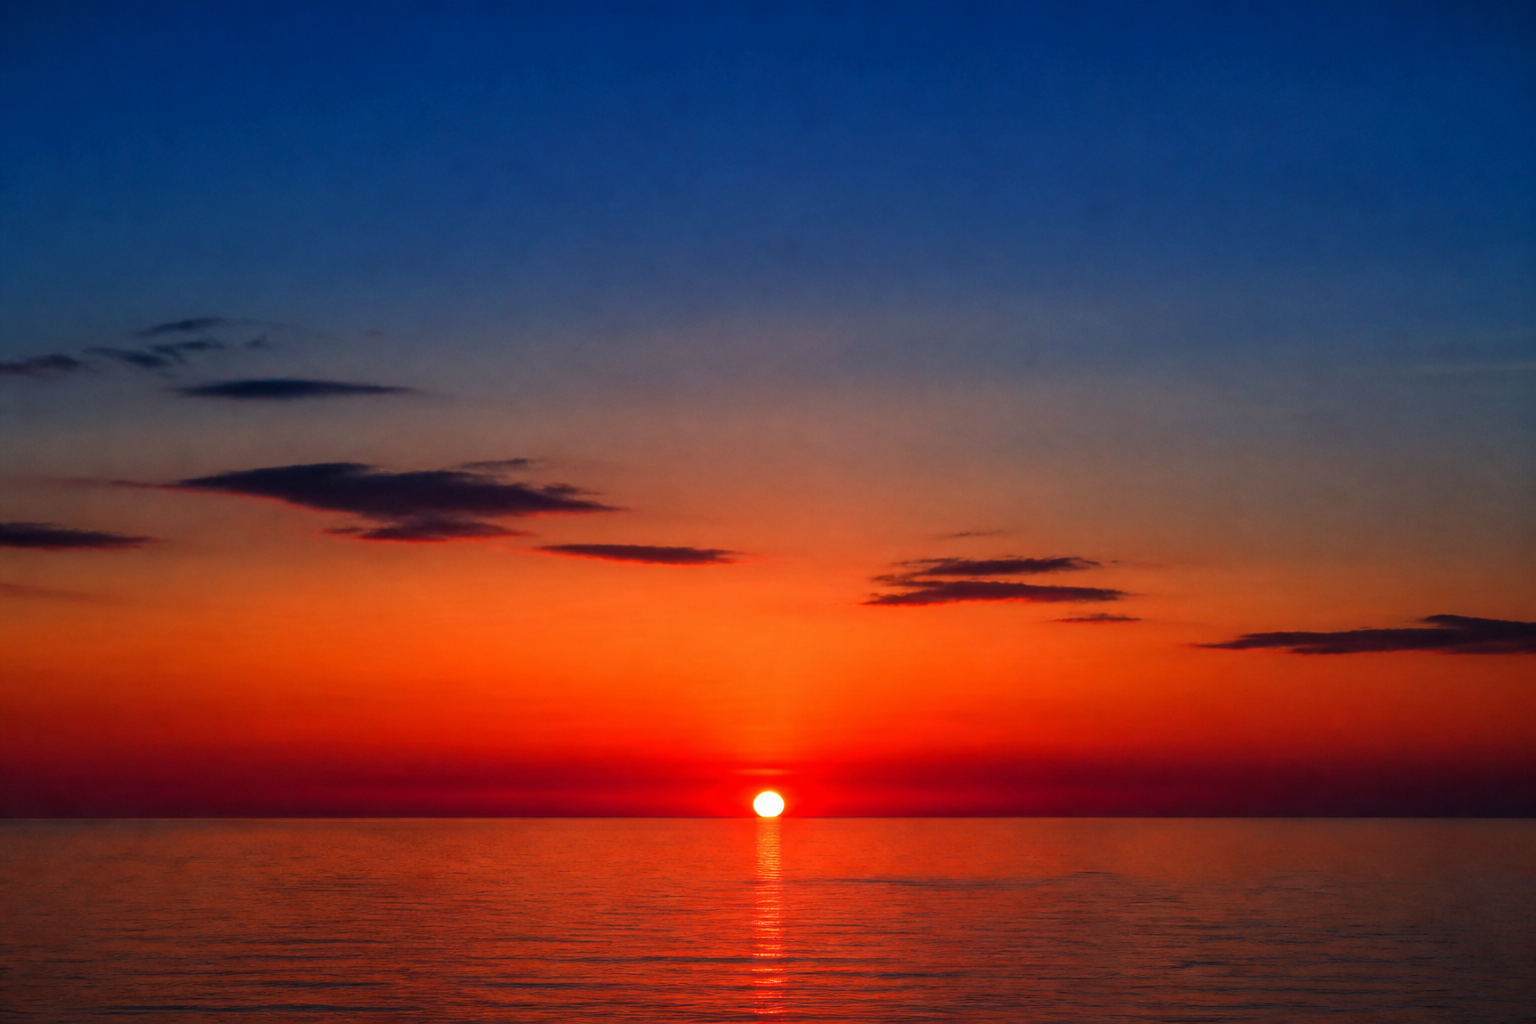
\includegraphics[width=0.58\linewidth]{images/book5/ai/b5-13-red-sunset.png}

{\small \omterm{thm:b3:perturbation-theory:corrections}{विक्षोभ सिद्धांत} के रूप में सूर्यास्त: हवा के अणु नीले प्रकाश को लाल से कहीं अधिक सहजता से प्रकीर्ण करते हैं (इस अध्याय के स्वर्ण-नियम-सजातीय $\omega^4$ के कारण), अतः क्षितिज पर का लंबा पथ नीले को छान लेता है और उसे किसी और के दोपहर के आकाश को भेज देता है।}
\end{omfigure}

\section{अभ्यास}

\begin{exercise}[$\star$]\label{exo:b3:perturbation-theory:1}
संदूक $[0, a]$ में कोई कण अतिरिक्त विभव $V(x) =
\lambda x/a$ अनुभव करता है। (क) हर स्तर का प्रथम-कोटि खिसकाव निकालिए
(किसी भी संदूक-अवस्था में $\langle x\rangle = a/2$ लीजिए --- इसका औचित्य दीजिए)।
(ख) यहाँ खिसकाव सब स्तरों के लिए एक ही क्यों है? (ग)
\emph{अंतरालों} का प्रथम-कोटि परिवर्तन क्या है, और
संक्रमण-आवृत्तियों की कोई माप इस विक्षोभ को पूरी तरह क्यों चूक सकती
है? (घ) प्रथम कोटि पर भरोसा कब बंद हो जाता है?
\end{exercise}

\begin{exercise}[$\star$]\label{exo:b3:perturbation-theory:2}
\cref{prop:b3:perturbation-theory:oscillator-field} की द्वितीय-कोटि
गणना पूरी कीजिए: $\hat x$ के आव्यूह-अवयव, दोनों पद, $n$ का कटना, और
वर्ग पूरा करने से मिला यथार्थ मेल। ऊर्जा का प्रथम-कोटि संशोधन लुप्त
होने पर भी \emph{अवस्था} का प्रथम-कोटि संशोधन लुप्त क्यों नहीं होता?
\end{exercise}

\begin{exercise}[$\star$]\label{exo:b3:perturbation-theory:3}
द्वि-स्तरीय \omterm{def:b3:hamiltonian-mechanics:hamiltonian}{हैमिल्टोनियन} $\begin{pmatrix}E_1 & v\\ v &
E_2\end{pmatrix}$, जहाँ $E_1 < E_2$ और $v$ वास्तविक। (क) यथार्थ
\omterm{def:b3:quantum-formalism:observable}{अभिलक्षणिक मान} ज्ञात कीजिए। (ख) $|v| \ll E_2 - E_1$ के लिए प्रसार कीजिए और
द्वितीय-कोटि सूत्र पहचानिए। (ग) दिखाइए कि स्तर ठेलते हैं: अंतराल सदा
$E_2 - E_1$ से अधिक रहता है। (घ) $E_1 = E_2$ पर: \omterm{thm:b3:perturbation-theory:corrections}{विक्षोभ सिद्धांत}
क्या देता है, यथार्थ उत्तर क्या देता है, और इस अध्याय की कौन-सी प्रमेय
उन्हें मिला देती है?
\end{exercise}

\begin{exercise}[$\star$]\label{exo:b3:perturbation-theory:4}
\cref{thm:b3:perturbation-theory:corrections} के लिए: (क) दिखाइए कि
प्रथम-कोटि अवस्था-संशोधन $\ket n$ के लांबिक है; (ख) दिखाइए कि
$\ket m$ का मिश्रण-गुणांक $V_{mn}/(E_n - E_m)$ है और
वैधता-कसौटी बताइए; (ग) कोई स्तर अपने निकटतम पड़ोसी से
$\qty{1}{eV}$ दूर है और उससे \qty{0.1}{eV} से युग्मित: मिश्रण की
प्रायिकता आँकिए; (घ) वही, पर \qty{10}{meV} के अंतराल के साथ ---
प्रसार का स्थान कौन-सा औज़ार लेगा?
\end{exercise}

\begin{exercise}[$\star\star$]\label{exo:b3:perturbation-theory:5}
अ-हरात्मक बंध। दोलक में $\hat V = \beta\hat x^3 + \gamma\hat x^4$
जोड़िए। (क) दिखाइए कि $x^3$ पद प्रथम कोटि पर किसी स्तर को नहीं खिसकाता
(सम-विषमता)। (ख) दिखाइए कि $x^4$ पद $\Delta E_n =
3\gamma(\hbar/2m\omega)^2(2n^2 + 2n + 1)$ देता है ($\hat x^4$ को
सोपान संकारकों में प्रसारित कीजिए; केवल ``संतुलित'' पद बचते हैं)। (ग) किसी वास्तविक बंध के लिए प्रभावी $\gamma$ ऋणात्मक होता है (कूप
बाहर की ओर नरम पड़ जाता है): दिखाइए कि तब स्तर-अंतराल $n$ के साथ
\emph{सिकुड़ता} है।
(घ) आणविक वर्णक्रमों की कौन-सी प्रेक्षित विशेषता
(\cref{exo:b3:harmonic-oscillator:4}) इससे बन जाती है?
\end{exercise}

\begin{exercise}[$\star\star$]\label{exo:b3:perturbation-theory:6}
वर्गाकार द्विविमीय संदूक में अपह्रासी युग्म $\ket{1,2},
\ket{2,1}$ को $\hat V = \lambda\,xy$ विक्षुब्ध करता है। (क) समझाइए कि
अ-अपह्रासी सिद्धांत क्यों विफल हो जाता है। (ख) $2\times2$ आव्यूह
निकालिए, उस युग्म में $\hat V$ का (समाकल गुणनखंडित हो जाते हैं; $\int_0^a
x\sin(\pi x/a)\sin(2\pi x/a)\dd x = -8a^2/9\pi^2$)। (ग)
विपाटन और सही शून्य-कोटि अवस्थाएँ ज्ञात कीजिए। (घ)
\cref{exo:b3:quantum-formalism:9} के सममिति-विश्लेषण से तुलना कीजिए:
सममिति ने कौन-सा उत्तर मुफ़्त में दे दिया था?
\end{exercise}

\begin{exercise}[$\star\star$]\label{exo:b3:perturbation-theory:7}
\omterm{ex:b3:perturbation-theory:stark}{स्टार्क प्रभाव}, रैखिक और द्विघातीय। (क)
\cref{ex:b3:perturbation-theory:stark} से $n = 2$ का विपाटन निकालिए,
$\mathcal E = \qty{2.5e6}{V/m}$ पर। (ख) मूल अवस्था कोई रैखिक खिसकाव
\emph{क्यों नहीं} दिखाती (दो कारण: सम-विषमता, और
कोई अपह्रासी साथी न होना)? (ग) उसका द्विघातीय खिसकाव ध्रुवणशीलता
परिभाषित करता है, $\Delta E = -\tfrac12\alpha\mathcal E^2$:
$\alpha \sim e^2a_0^2/E_{\text{I}}$ आँकिए और उसका मान
$a_0^3$ के मात्रकों में निकालिए (यथार्थ उत्तर $4.5\,a_0^3 \times
4\pi\varepsilon_0$ है)। (घ) पदार्थ का कौन-सा रोज़मर्रा का गुण ---
उसकी परावैद्युत अनुक्रिया --- आपने अभी परमाणु-स्तर पर निकाल लिया?
\end{exercise}

\begin{exercise}[$\star\star$]\label{exo:b3:perturbation-theory:8}
स्वतःस्फूर्त उत्सर्जन (एक स्वीकृत निवेश के साथ): कोई उत्तेजित अवस्था
$A = \omega^3|d_{fi}|^2/3\pi\varepsilon_0\hbar c^3$ पर क्षय होती है,
जहाँ $d_{fi} = e\bra f\hat z\ket i$ जैसे आव्यूह-अवयव
द्विध्रुव तय करते हैं। (क) हाइड्रोजन के $2p \to 1s$ के लिए: $|d| \approx 0.74\,
ea_0$ और $\lambda = \qty{121.6}{nm}$ के साथ $A$ और
जीवनकाल निकालिए। (ख) उसे सोडियम की D रेखा तक मापित कीजिए। (ग)
अतिसूक्ष्म 21 cm संक्रमण तक मापित कीजिए ($|d| \to$ कोई चुंबकीय आघूर्ण,
और दर एक और $\alpha^2$-जैसे गुणक से नीचे; $A \approx
\qty{2.9e-15}{s^{-1}}$ स्वीकार कीजिए): ``एक करोड़ वर्ष'' जाँचिए। (घ)
$\omega^3$ से: पराबैंगनी रेखाएँ तेज़ और रेडियो रेखाएँ शाश्वत क्यों हैं,
और इससे \omterm{ex:b3:spin-two-level:hyperfine}{21 cm रेखा}
\emph{भविष्यवाणी योग्य} पर किसी प्रयोगशाला में लगभग असंसूचनीय क्यों बन गई?
\end{exercise}

\begin{exercise}[$\star\star$]\label{exo:b3:perturbation-theory:9}
चयन-नियम, समाकलों के रूप में। (क) सम-विषमता से दिखाइए कि $\bra{100}\hat z\ket{200} =
0$। (ख) दिखाइए कि $\bra{100}\hat z\ket{21m} = 0$, जब तक $m =
0$ न हो ($\varphi$ का समाकल)। (ग) इससे निकलने वाले नियम $\Delta
l = \pm1$, $\Delta m = 0, \pm1$ बताइए और उनका भौतिक पाठ भी (अर्थात्
फ़ोटॉन का चक्रण)। (घ) $2s$ अवस्था किसी द्विध्रुव-मार्ग से
$1s$ तक नहीं पहुँच सकती: इससे उसके जीवनकाल की क्या भविष्यवाणी होती है,
और प्रकृति वास्तव में कौन-सा ``वर्जित'' दो-फ़ोटॉन मार्ग लेती है?
\end{exercise}

\begin{exercise}[$\star\star\star$]\label{exo:b3:perturbation-theory:10}
ध्रुवणशीलता, ईमानदारी से। किसी क्षेत्र में हाइड्रोजन की मूल अवस्था का
द्वितीय-कोटि खिसकाव $\Delta E = -e^2\mathcal E^2\sum_{m\neq
0}|\bra m\hat z\ket 0|^2/(E_m - E_0)$ है। (क) हर हर के स्थान पर सबसे
छोटा अंतराल $E_2 - E_1 =
\tfrac34 E_{\text{I}}$ रखकर और संवृत्ति-संबंध $\sum_m|\bra
m\hat z\ket0|^2 = \langle z^2\rangle_0 = a_0^2$ काम में लाकर योग को
बाँधिए: $\alpha
\le \tfrac{16}3\,a_0^3$ निकालिए ($4\pi\varepsilon_0$ वाले
गाउसीय-शैली मात्रकों में)। (ख) यथार्थ $\tfrac92 a_0^3$ से तुलना कीजिए।
(ग) $\alpha$ से वायुमंडलीय घनत्व पर हाइड्रोजन गैस का अपवर्तनांक
आँकिए ($n - 1 \approx N\alpha/2\varepsilon_0
\cdot e^2\dots$ --- $n - 1 = N\alpha_{\text{SI}}/2
\varepsilon_0$ लीजिए) और मापे गए $\num{1.3e-4}$ से तुलना कीजिए।
(घ) एक वाक्य में वह शृंखला बताइए, परमाणु $\to$ ध्रुवणशीलता
$\to$ अपवर्तन, जिस पर सप्ताहांत समस्या का भाग II सवारी करेगा।
\end{exercise}

\begin{exercise}[$\star\star\star$]\label{exo:b3:perturbation-theory:11}
बचे हुए कटाव और मंद झाड़ू। किसी द्वि-स्तरीय तंत्र की नग्न
ऊर्जाएँ $\pm\lambda t$ हैं, जो $t = 0$ पर कटती हैं, और जिन्हें $v$
युग्मित करता है। (क) $t$ के सामने यथार्थ स्तरों का रेखाचित्र बनाइए:
$2|v|$ अंतराल वाला एक बचा हुआ कटाव। (ख) यदि झाड़ू \emph{मंद} हो, तो
तंत्र निचले वक्र का अनुसरण करता है (रुद्धोष्म प्रमेय, स्वीकृत): वह
अंत में किस अवस्था में पहुँचता है? (ग) लांडाउ--त्सेनर कसौटी अंतराल
वाले क्षेत्र को पार करने का समय, $\sim v/\lambda$, भीतरी घड़ी
$\hbar/v$ से तुलती है: रुद्धोष्म अनुसरण की शर्त दीजिए। (घ) दो
उपयोग: किसी मंद चहचहाहट से अंतरित की गई क्यूबिट-अवस्था; और नाभिकों के
बीच आवेश उछालता कोई परमाणु-संघट्ट --- इनमें से किसी एक को
दो वाक्यों में समझाइए।
\end{exercise}

\begin{exercise}[$\star\star\star$]\label{exo:b3:perturbation-theory:12}
द्वितीय कोटि निराशावादी है, और कुछ अन्य प्रमेय। (क) सिद्ध कीजिए कि
\emph{मूल} अवस्था का द्वितीय-कोटि संशोधन सदा
ऋणात्मक होता है। (ख) इससे (और
\cref{exo:b3:harmonic-oscillator:10} से) निष्कर्ष निकालिए कि
मूल-अवस्था परमाणुओं के बीच वान डर वाल्स बल सदा आकर्षक क्यों हैं। (ग)
दिखाइए कि प्रथम-कोटि सिद्धांत हर मूल-अवस्था ऊर्जा को
\emph{अधिक आँकता} है: वह एक विचरण-बंध है (अविक्षुब्ध अवस्था को
परीक्षण-अवस्था लेकर $\bra{\psi_0}\hat
H\ket{\psi_0}$ का मान निकालिए)। (घ)
\cref{ex:b3:perturbation-theory:stark} पर एक संगति-जाँच:
\emph{रैखिक} \omterm{ex:b3:perturbation-theory:stark}{स्टार्क प्रभाव} (क) का उल्लंघन क्यों नहीं है?
\end{exercise}

\section{समस्या: आकाश का रंग}

\begin{problem}[{सप्ताहांत समस्या --- विक्षुब्ध परमाणुओं से रैले
प्रकीर्णन}]\label{pb:b3:perturbation-theory:1}
दिन का आकाश नीला, सूर्यास्त लाल और बादल सफ़ेद क्यों है? पूरा
उत्तर इसी अध्याय से होकर जाती एक शृंखला है: कोई प्रकाश-तरंग हवा के हर
अणु को विक्षुब्ध करती है; प्रेरित द्विध्रुव फिर से विकिरण करता है (वर्ष
2 के खंड का द्विध्रुव विकिरण); और व्यतिकरण तय करता है
कि क्या बचेगा। आँकड़े: हवा की आणविक ध्रुवणशीलता
$\alpha/4\pi\varepsilon_0 \approx \qty{2.2e-30}{m^3}$; संख्या-घनत्व
$N = \qty{2.5e25}{m^{-3}}$; दृश्य परिसर
$450$--\qty{700}{nm}।

\medskip\noindent\textbf{भाग I --- विक्षुब्ध अणु।}
\begin{enumerate}
  \item कोई स्थैतिक क्षेत्र $\mathcal E$ किसी अणु की मूल अवस्था को
        $-\tfrac12\alpha\mathcal E^2$ जितना खिसका देता है: इस
        कथन को द्वितीय-कोटि \omterm{thm:b3:perturbation-theory:corrections}{विक्षोभ सिद्धांत} से जोड़िए (कौन-सा
        सूत्र, और ऋणात्मक क्यों?)।
  \item वही $\alpha$ प्रेरित द्विध्रुव $p =
        \alpha\mathcal E$ देता है: सूर्य-प्रकाश के क्षेत्र $\mathcal E \sim
        \qty{800}{V/m}$ के लिए किसी एक नाइट्रोजन अणु का प्रेरित
        द्विध्रुव निकालिए और उसकी तुलना $ea_0$ से कीजिए।
  \item जिन अणुओं के इलेक्ट्रॉनिक संक्रमण पराबैंगनी में हैं, उनके
        लिए प्रकाशिक क्षेत्र (आवृत्ति $\num{5e14}$ Hz) को
        \emph{स्थैतिक} ध्रुवणशीलता से क्यों निपटाया जा सकता है?
        ($\hbar\omega$ की तुलना अंतराल से कीजिए; यह स्वर्ण-नियम के
        हर की अनुनाद-से-बहुत-दूर वाली सीमा है।)
  \item कोई दोलायमान द्विध्रुव $p_0\cos\omega t$ औसत शक्ति
        $P = p_0^2\omega^4/12\pi\varepsilon_0c^3$ विकिरित करता है
        (वर्ष 2 का खंड)। $p_0 = \alpha\mathcal
        E_0$ के साथ मिलाकर: नियत प्रदीपन पर प्रकीर्ण शक्ति
        $\omega$ पर कैसे निर्भर करती है?
  \item \qty{450}{nm} और \qty{700}{nm} पर प्रकीर्ण शक्तियों का
        अनुपात निकालिए।
  \item एक वाक्य में: आकाश नीला क्यों है, बैंगनी क्यों नहीं
        (दो अवयव: सूर्य का वर्णक्रम, जो बैंगनी की ओर गिरता है, और
        आँख की सुग्राहिता)?
\end{enumerate}

\medskip\noindent\textbf{भाग II --- एक अणु से पूरे
आकाश तक।}
\begin{enumerate}[resume]
  \item प्रकीर्णन की अनुप्रस्थ काट $\sigma =
        \dfrac{8\pi}{3}\Big(\dfrac{\alpha}{4\pi\varepsilon_0}
        \Big)^2\dfrac{\omega^4}{c^4}$ निकलती है: उसकी विमाएँ जाँचिए
        और \qty{550}{nm} पर उसका मान निकालिए।
  \item क्षीणन-लंबाई $\ell = 1/N\sigma$ है: \qty{550}{nm} पर उसका
        मान निकालिए और वायुमंडल की मोटाई से तुलना कीजिए
        (समुद्र-तल घनत्व पर $\sim\qty{8}{km}$ के तुल्य)।
  \item \qty{450}{nm} बनाम \qty{700}{nm} पर किसी ऊर्ध्वाधर
        सूर्य-किरण का कितना अंश प्रकीर्ण होकर बाहर जाता है?
        ($1 -
        \eu^{-L/\ell}$ लीजिए, जहाँ $L = \qty{8}{km}$।)
  \item सूर्यास्त पर पथ तीस गुना लंबा होता है: नीले का बचाव फिर से
        निकालिए और नीचे उतरे सूर्य का रंग समझाइए ---
        तथा उस प्रकाश का भी जो किसी चंद्रग्रहण में चंद्रमा को लाल कर
        देता है।
  \item सूर्य से $90^\circ$ पर आकाश का प्रकाश \emph{ध्रुवित} क्यों
        होता है (द्विध्रुव के विकिरण-प्रतिरूप को स्मरण कीजिए:
        द्विध्रुव की अपनी अक्ष के अनुदिश कोई उत्सर्जन नहीं)?
  \item कहा जाता है कि मधुमक्खियों और वाइकिंगों ने इसी ध्रुवण से
        दिशा पाई: बादल छाया दिन उसका क्या कर देता है, और
        क्यों?
\end{enumerate}

\medskip\noindent\textbf{भाग III --- आकाश और अधिक चमकीला क्यों
नहीं।}
\begin{enumerate}[resume]
  \item एक विरोधाभास: किसी पूर्णतः एकसमान माध्यम में पड़ोसी
        आयतन-अवयवों की लहरें बगल की ओर विनाशी व्यतिकरण करती हैं,
        और \emph{कोई} प्रकाश प्रकीर्ण ही न होता (केवल अपवर्तन
        बचता)। हवा की एकसमानता वास्तव में क्या तोड़ता है --- यादृच्छिक
        रूप से बँटा हुआ क्या है?
  \item किसी आदर्श गैस के घनत्व-उतार-चढ़ाव स्वतंत्र अणुओं की प्रकीर्ण
        तीव्रताओं को \emph{जुड़ने} देते हैं: बताइए कि
        स्वतंत्रता (यादृच्छिक स्थितियाँ, तरंगदैर्घ्य-पैमाने के
        अंतराल) विनाशी व्यतिकरण को क्यों मार देती है।
  \item \qty{550}{nm} पर अपने $\ell$ से: एक स्वच्छ दिन का
        वायुमंडल सूर्य-प्रकाश का कितना अंश प्रकीर्ण करता है --- क्या
        वह संख्या सूर्य-बिंब के सामने आकाश की रोज़मर्रा की चमक से मेल
        खाती है?
  \item किसी बादल की बूँद (\qty{10}{\micro m}) में एक तरंगदैर्घ्य के
        भीतर $\sim10^{12}$ अणु होते हैं: उनकी लहरें
        \emph{संसक्त} रूप से जुड़ती हैं। तब प्रकीर्ण शक्ति अणु-संख्या
        के साथ कैसे मापित होती है, और $\omega^4$ वाला
        रंग-चयन क्यों लुप्त हो जाता है (सारी तरंगदैर्घ्य प्रबल रूप से
        प्रकीर्ण होती हैं): बादल किस रंग का है?
  \item दूध, कुहरा और सफ़ेद रंग इसी कारण सफ़ेद हैं: व्यापक नियम
        बताइए --- $\lambda$ के सामने छोटे प्रकीर्णक प्रकाश को रंग देते
        हैं, और $\lambda$ के सामने बड़े प्रकीर्णक उसे सफ़ेद कर देते हैं।
  \item क्रांतिक दुग्धाभा: किसी द्रव के क्रांतिक बिंदु के पास
        (वर्ष 1 के खंड के अवस्था-परिवर्तन अध्याय, और आगे
        \cref{ch:b3:phase-transitions}) घनत्व-उतार-चढ़ाव प्रकाशिक पैमानों तक बढ़ जाते हैं और
        तरल दूधिया हो जाता है: इसे मद 13 से जोड़िए।
\end{enumerate}

\medskip\noindent\textbf{भाग IV --- शृंखला, पूरी की हुई।}
\begin{enumerate}[resume]
  \item आगे की ओर प्रकीर्ण लहरें \emph{नहीं} कटतीं: वे पुंज के साथ
        व्यतिकरण करती हैं और उसकी कला धीमी कर देती हैं --- अर्थात्
        अपवर्तनांक। $n - 1 = N\alpha/2\varepsilon_0$
        ($\alpha$ SI में) से हवा के लिए $n - 1$ का मान निकालिए और
        मापे गए \num{2.9e-4} से तुलना कीजिए।
  \item इस तरह एक ही नियतांक $\alpha$, जिसे द्वितीय-कोटि
        \omterm{thm:b3:perturbation-theory:corrections}{विक्षोभ सिद्धांत} से निकाला गया, एक साथ तीन परिघटनाएँ तय कर
        देता है: उन्हें गिनाइए (किसी स्थैतिक क्षेत्र में खिसकाव;
        आकाश का नीलापन; हवा में प्रकाश का मुड़ना)।
  \item ओज़ोन का अवशोषण, ऐरोसॉल और बहु-प्रकीर्णन असली आकाशों को
        जटिल बना देते हैं: हर एक का एक प्रेक्षणीय बताइए
        (गोधूलि के रंग; दूधिया क्षितिज; सूर्यास्त के बाद शिखर-बिंदु
        पर आकाश की बची हुई चमक)।
  \item वायुहीन चंद्रमा दिन में \emph{काला} आकाश क्यों ढोता है ---
        और उसकी सतह से लिए गए हर छायाचित्र ने इससे हमारे आकाश के
        उद्गम के विषय में क्या पुष्ट किया?
  \item मंगल का दिन का आकाश हलका भूरा है और उसके सूर्यास्त
        \emph{नीले}: उसकी पतली हवा कम प्रकीर्ण करती है, और यह काम
        उसमें लटके माइक्रोमीटर धूल-कण करते हैं। मद 18 के नियम से
        समझाइए कि धूल रंग का तर्क कैसे उलट देती है।
  \item एक्स-किरणों के लिए $\hbar\omega$ हर आणविक संक्रमण से कहीं
        अधिक है: तब इलेक्ट्रॉन ऐसे अनुक्रिया करते हैं मानो मुक्त हों,
        और प्रकीर्णन (थॉमसन) अपना $\omega^4$ खो देता है। उस परिसर
        में ``आकाश-नीला'' क्रियाविधि का क्या होता है --- और वही सपाट
        अनुक्रिया एक्स-किरणों को इलेक्ट्रॉन-घनत्व की स्वच्छ जाँच
        क्यों बना देती है?
  \item नामित परिणाम का सार लिखिए: $\qty{2.2e-30}{m^3}$ की कोई
        ध्रुवणशीलता, वर्ग करके $\omega^4$ से गुणा की हुई,
        हरे में \qty{60}{km} के पैमाने की प्रकीर्णन-लंबाई देती है
        --- इतनी लंबी कि दोपहर का आकाश कोमल रहे, और इतनी छोटी कि
        सूर्यास्त लाल हो जाएँ तथा आकाश नीला रहे, और वह भी चालित
        द्विध्रुवों के जंगल जैसे ध्रुवण-प्रतिरूप के साथ।
\end{enumerate}
\end{problem}
